\documentclass[11pt]{article}
\usepackage[english]{babel}
\usepackage[utf8x]{inputenc}
\usepackage{amsmath}
\usepackage{graphicx}
\usepackage{fullpage}
\usepackage[colorinlistoftodos]{todonotes}
\usepackage[numbers, sort&compress]{natbib}
\usepackage[version=3]{mhchem}
\usepackage{setspace}
\usepackage[ampersand]{easylist}
\usepackage[obeyspaces]{url}

\onehalfspacing

\title{Representing chemical data from Reaction Mechanism Generator (RMG) in a relational database}

\author{Belinda Slakman}

\begin{document}
\maketitle

\section{Introduction}

Reaction Mechanism Generator (RMG) is an open-source software used to build detailed chemical kinetic models, given starting chemical species and process conditions such as initial concentrations, temperature, pressure, and solvent \cite{RMGPy}. RMG, written in Python, is generally used to build models for hydrocarbon combustion, but recent additions allow some functionality for oxygenated biofuels, liquid-phase reactions, and silicon hydrides. For generating these models, a large number of thermodynamic and kinetic parameters must be known or estimated from known values. The parameters that various users and developers have added to RMG are stored in a database.

Currently, RMG's database is stored in a series of Python files. Each entry in the database is associated with a particular chemical species or a reaction. The structure is similar to a key-value structure where each entry has a label and a set of values associated. Figure \ref{fig:thermo_entry} shows an example of an entry in a thermodynamic library.

\begin{figure}[h]
\centering
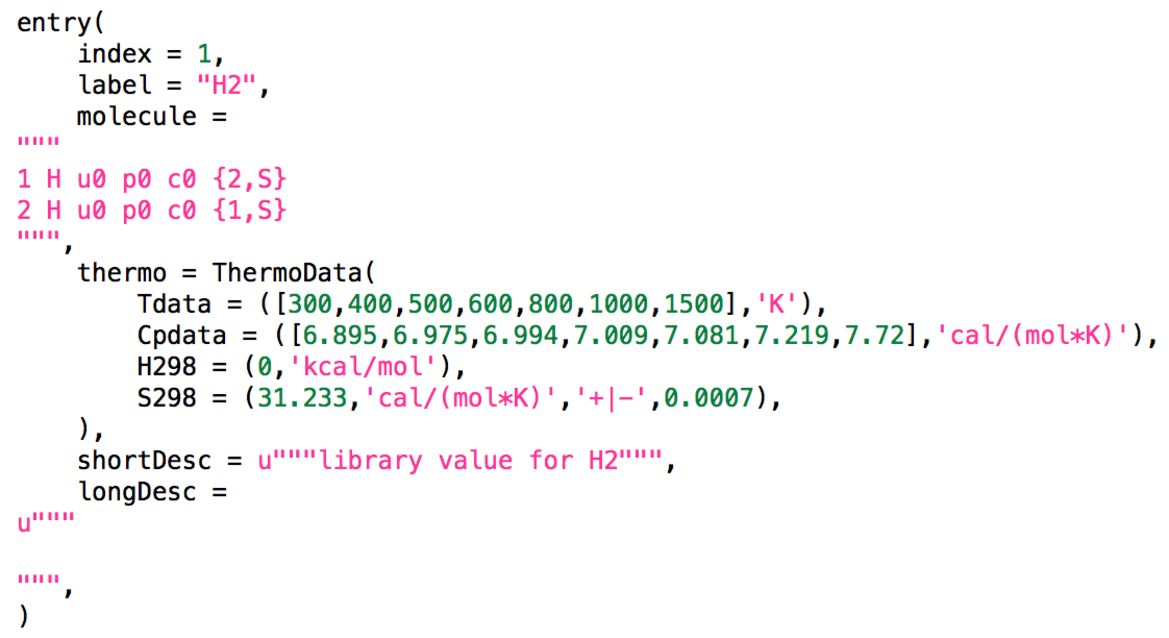
\includegraphics[width=0.75\textwidth]{thermo_entry.pdf}
\caption{\label{fig:thermo_entry} Example of an entry from a thermodynamic library in RMG-database. The entry contains an index, label, adjacency list, thermodynamic data, and comments.}
\end{figure}

The problem with the RMG database's current structure is that data is looked up constantly on-the-fly during the course of a simulation. When we encounter a new species, we must look up its thermodynamic and solvation data in separate libraries. Furthermore, if multiple thermodynamic libraries were specified in the input file, we will only use the value from the first library listed, even if the species exists in other libraries with different thermodynamic values. The index associated for each entry in a library is also relatively meaningless. Another issue is that chemical species cannot be specified uniquely; they are specified with a non-canonical label and an adjacency list. Graph matching algorithms are used to compare the adjacency lists. It would be desirable to both reduce the number of lookups and increase the speed of the lookups by simplifying the database currently used.

A relational database structure could solve some of these issues. Relational data lookup is fast, and the data we are working with is mainly in text form. A relational database can also better represent relationships between data; molecules may appear in multiple reactions in kinetics libraries, as well as be associated with thermodynamic data in several libraries, and have associated solvation data. Furthermore, users who are not performing an RMG simulation, but have general questions about the data available or about some reactions or chemical species, can easily and quickly perform queries on this relational database.

\section{Description of project aims}
The aims of the term project will be described below.
\subsection{Demonstrate web scraping concepts to retrieve parameters  from the RMG database}
In addition to the Python files, the RMG-database is also available on the web at both \url{rmg.coe.neu.edu/database} and \url{rmg.mit.edu/database}. To demonstrate the web scraping methods from this course with the XML and RCurl packages in R, thermodynamic, kinetic and solvation data will be scraped from various libraries and sorted into data frames.
\subsection{Restructure parts of the RMG database into a relational database}
By reorganizing data and using the SQLite package in R, the data collected in the first aim will be organized into a relational database that satisfies third normal form.
\subsection{Perform queries of data of interest to someone working with RMG or with chemical data}
Ability to query the database, again using the SQLite package in R, will be demonstrated. From the result of these queries we can understand the strengths and weaknesses of using a relational database structure to represent RMG's database.

\section{Web Scraping}
Methods written to scrape thermodynamic, kinetic and solvation data are contained in the attached file \path{RMGWebScraping.R}. This file depends on the packages RCurl and XML. It contains three methods: \texttt{ScrapeRMGThermo()}, \texttt{ScrapeRMGKineticsFromLibrary()}, and \texttt{ScrapeRMGSolvation()}, each returning a data frame of the quantities of interests. These will be described in detail below.

\subsection{Thermodynamics}
The thermodynamic data can come from two different source types, libraries or groups, with each type having different libraries or sets of groups. For example, thermodynamic libraries include sets of parameters determined from quantum mechanics calculations, such as "DFT\_QCI\_Thermo", or from other groups' work, including "GRI-Mech3.0". Each library be associated with a different research group or set of chemical species. Thermodynamic group values belong to molecular structure groups that make up a chemical species, such as radicals or rings. Despite differences between full molecules and groups, the webpages are structured mostly the same, so we have the option of scraping differently. However, the groups are listed in a tree based on molecular structure allowing for easier lookup; we cannot replicate this tree in a relational database.

The RCurl package is used to retrieve URLs and the XML package is used to process the webpage and retrieve nodes (using xslt language). The number of species is found by retrieving the last node on the library or group page; this is useful because we can then pre-allocate vectors of values, saving on computational time when looping through each molecule or group. The information retrieved and parsed includes the molecule label (name or chemical formula), its adjacency list, the enthalpy of formation (Hf), entropy of formation (Sf), and heat capacity at two different temperatures (Cp\_300 and Cp\_1000). Hf, Sf, Cp\_300, and Cp\_1000 are only retrieved if the thermo is in the format "Group additivity". One could imagine having other scraping functions for thermo given in different forms, such as NASA polynomials, but for simplicity only one is included here. Rows of all 'NA' values, meaning no webpage existed for a particular index so it was skipped, are removed before returning the data frame. An example of a data frame of thermodynamic library data is given in Figure \ref{fig:thermo_df}.

\begin{figure}[h]
\centering
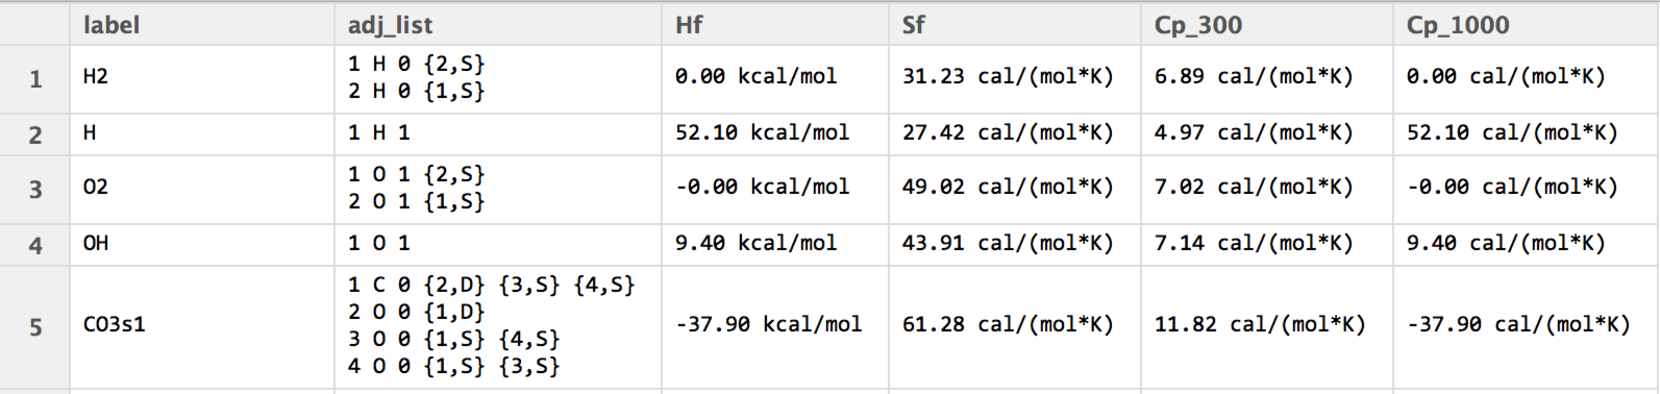
\includegraphics[width=0.75\textwidth]{thermo_df.pdf}
\caption{\label{fig:thermo_df} Result of running the scraping method \texttt{ScrapeRMGThermo('libraries', 'primaryThermoLibrary')}. Only the first five entries are shown.}
\end{figure}

\subsection{Kinetics}

The web scraping protocol for RMG kinetics is similar to that for thermodynamics, but we do not include an option for scraping the kinetics groups since the format is very different than that of the libraries. The values scraped are the reactants (by name or chemical formula, up to 3), products (up to 3), and Arrhenius kinetics parameters including the pre-exponential factor (A), temperature exponent (n), and activation energy ($\mathrm{E_A}$). If kinetics is not Arrhenius, we skip the scraping for that reaction; again, one could add different protocols for scraping kinetics of different formats.

\begin{figure}[h]
\centering
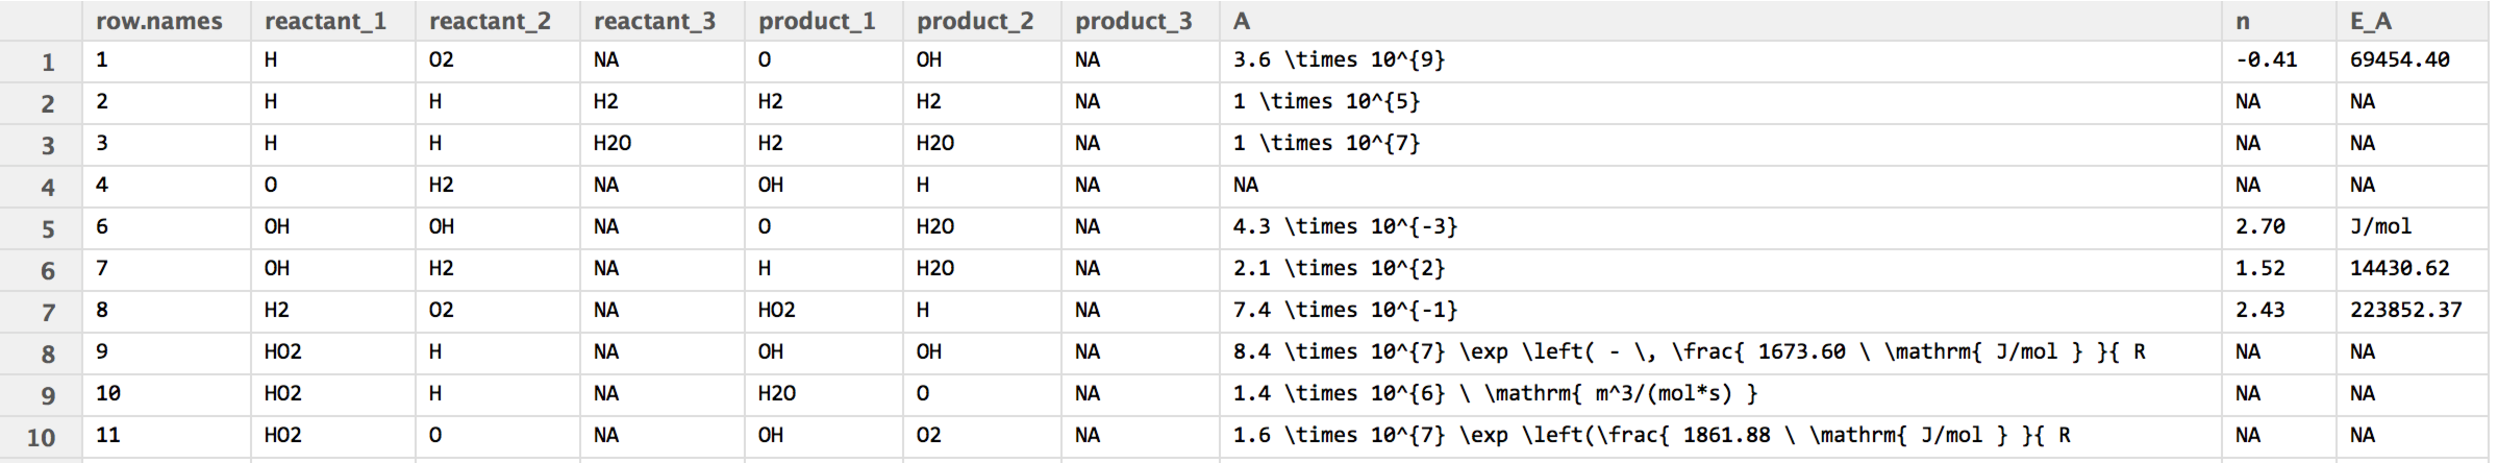
\includegraphics[width=0.9\textwidth]{kinetics_df.pdf}
\caption{\label{fig:kinetics_df} Result of running the scraping method \texttt{ScrapeRMGKineticsFromLibrary('GRI-Mech3.0')}; only the first five entries are shown. Note that the cleaning of the data did not work for all of the kinetic parameters.}
\end{figure}

The data frame created from the web scraping is shown in Figure \ref{fig:kinetics_df}. Note that the text processing fails on separating some of the Arrhenius parameters into A, n and $\mathrm{E_A}$; using a different web scraping tool could make the data cleaning easier.

\subsection{Solvation}

Scraping the solvation data is similar to thermodynamics and kinetics, but it is easier because there is only one solute library available in RMG so it is scraped by default. The solute parameters (S, B, E, L, A and V) are coefficients in a linear solvation energy relationship that relates gas and solution phase thermodynamics for a chemical species. A portion of the data frame resulting from scraping the solvation library is illustrated in Figure \ref{fig:solvation_df}.

\begin{figure}[h]
\centering
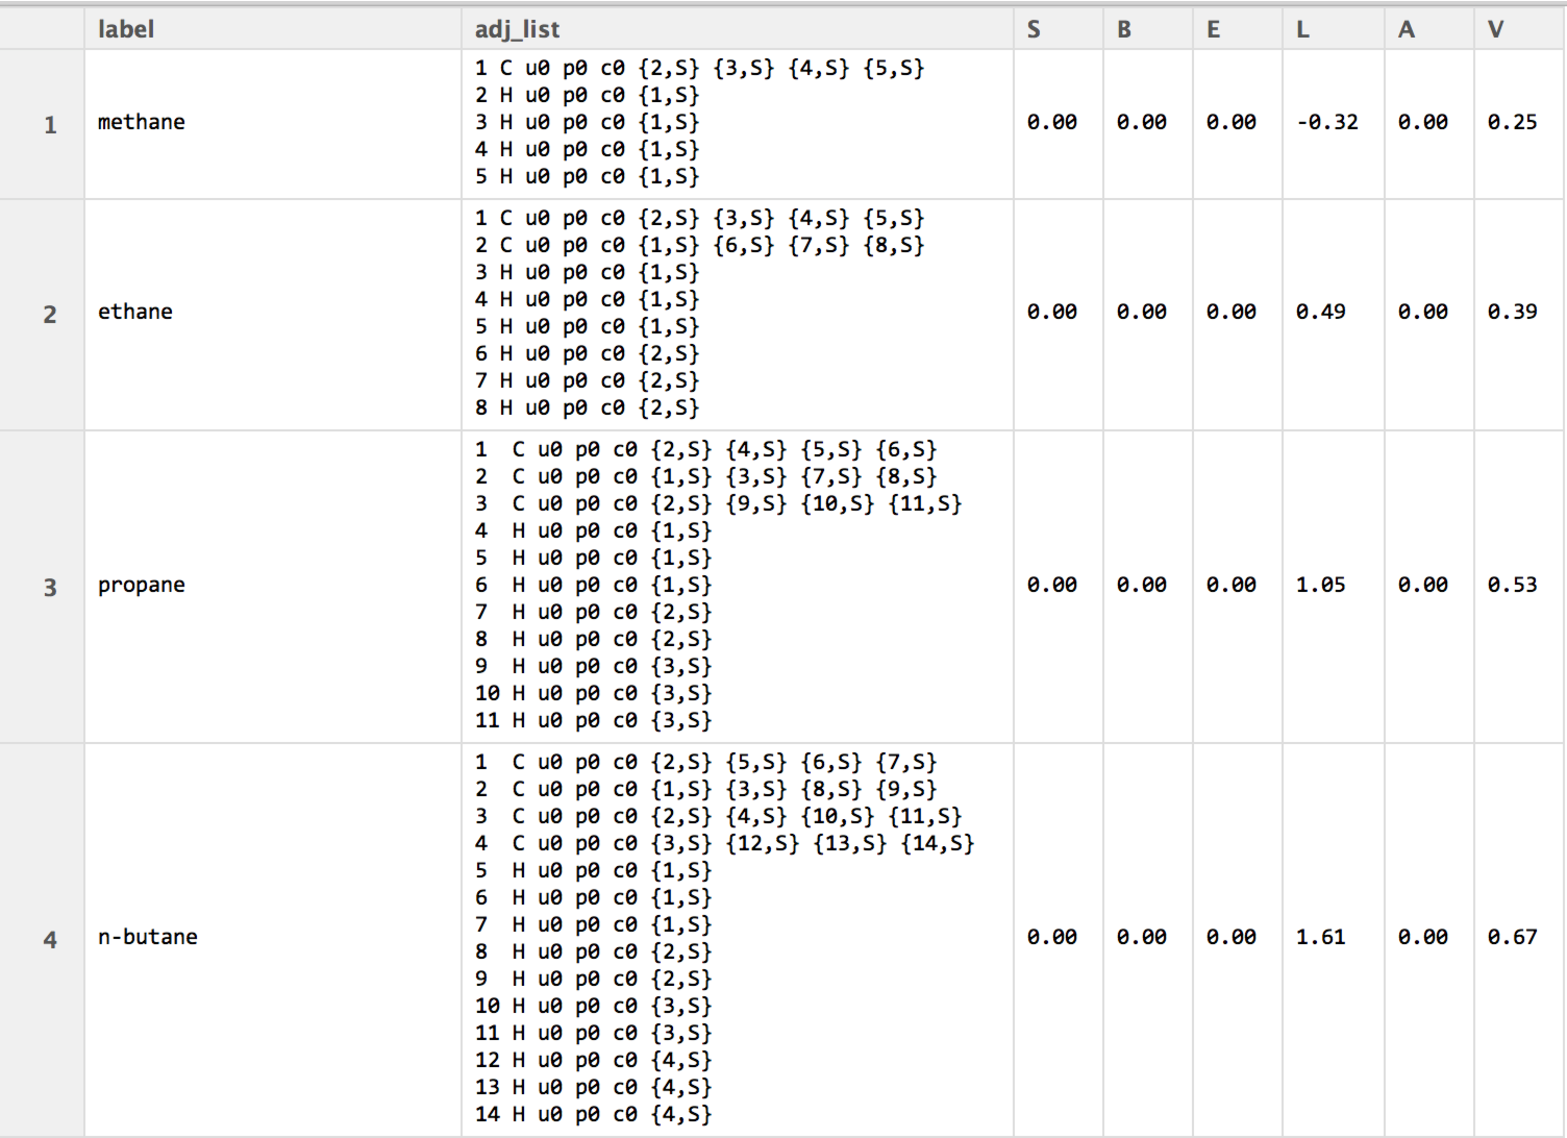
\includegraphics[width=0.75\textwidth]{solvation_df.pdf}
\caption{\label{fig:solvation_df} Result of running the scraping method \texttt{ScrapeRMGSolvation()}.}
\end{figure}

\section{Transformation into a relational database}
Data manipulations were performed in R to translate the scraped data into three tables for a relational database. The manipulations, and the following queries were done in the attached file \path{RMGDatabase.R}. Examples of three thermodynamic libraries, three kinetic libraries, and the solvation library were scraped for data. An explanation of each table, and how the database satisfies third normal form, is below. 
\subsection {Thermodynamic data table}
The primary keys in the thermodynamic table are the species identifier, \emph{label}, and the thermodynamic library it belongs to, \emph{thermoLibraryName}. Together, these keys uniquely specify a single thermodynamic entry, as the same molecule can only appear once in a thermo library (although it can appear in several libraries). The table also contains thermodynamic parameters.

\subsection{Molecule and solvation data table}
The second table contains the each molecule's label, adjacency list and its solvation data. The primary key is the \emph{label}. The adjacency list and the solvation data should be unique to a molecule, since there is only solute library and the adjacency list for a given molecule should give the same chemical graph. Note that this does NOT mean that the adjacency list string is unique for a given molecule, because atoms can be specified in any order. This is why we select unique rows from the resulting table, since we can have the same molecule multiple times with different adjacency lists (that mean the same thing, so it doesn't matter what row we keep). 

\subsection{Kinetic data}
The table containing the kinetic data contains an index, the name of the kinetics library, the reactants and products, and the Arrhenius kinetic data. The \emph{index} and the \emph{kineticsLibraryName} uniquely specify the reaction and are used as the primary key. This allows a reaction with the same reactants and products, but different kinetics, to be listed more than once.

\subsection{Satisfying 3NF}
The database satisfies 1NF since each has a primary key, and no table has multiple values for a single column. Also, each column's value depends on the primary key of the table. This is why adjacency list and solute data were placed in the same table, since neither of these depends on the thermodynamic or kinetic library the molecule is in.

2NF applies to the thermodynamics and kinetics tables, which have multiple columns as primary keys. The values in the other columns in each table definitely depend on the thermodynamic library or kinetic library, respectively; a label or an index was not sufficient since a single molecule or reaction can appear in multiple libraries.

The database also satisfies 3NF because no columns are dependent on anything but the primary keys. One could argue that some reaction rates are known so well that the Arrhenius parameters are dependent on the reactants and products themselves and not the index and reaction library; however, inconsistencies still occur between different experimental and calculation methods (and no reaction rate is known that accurately!)

\section{Querying the database}

Chemical data queries are performed in the file \path{RMGDatabase.R} via SQL SELECT statements. A summary of the results follows:
\begin{easylist}[itemize]
& OH appears in both the primaryThermoLibrary and DFT\_QCI\_Thermo libraries.
& The chemical species that appear in more than one library are H2, O2, and OH. These queries are useful, because we can compare the thermodynamic parameters in each and if there is a large discrepancy, it motivates further experimentation or calculation.
& In the three libraries, H2 appears as a reactant or product 94 times. Knowing how many times a species appears also can motivate further research.
& 62 reactions in GRI-Mech3.0, 162 in Glarborg/C3, and 23 in Sulfur/DMS have kinetics in Arrhenius format. Note that these numbers may be incorrect due to faulty scraping.
& None of the molecules in the primaryThermoLibrary contain solvation data. This is not actually true, but why this result occurs will be discussed.
\end{easylist}

\section{Discussion}
\label{sec:discussion}

While web scraping using XML in R and subsequent cleaning of data could be done reasonably well for thermodynamic and solvation data, we had an issue with the Arrhenius parameters. To this end, one of the web scraping tools in the class might be better suited to capture these parameters; though they are less customizable, they require less user input. Kimono was the option I found easiest to use during the course exploration of tools.

For both scraping and manipulating the data into a relational database, we found that libraries of data represented by entire molecules were easier to deal with than group data, in which values are defined by molecular structure groups. Because groups are represented by hierarchical trees, it would be beneficial to represent this tree in a graph database where relationships, such as parent and child, are known between nodes.

Querying of the database succeeded for most of the queries; however, it failed when we looked for solvation data for molecules in a particular thermodynamic library. This failure is due to a flaw in the keys used to represent molecules. We inherently assume that the label representation of a molecule is the same across all libraries, but the way RMG actually does these comparisons is through graph matching algorithms of the adjacency lists. However, the solvation library was created with name labels (e.g. methane) and the thermodynamic and kinetic libraries mainly use chemical formula labels (e.g. CH4), which is why our query failed. Graph matching introduces a speed limitation in RMG, because if we could instead do simple string comparison, all queries would be much quicker (regardless of the database structure used). However, although strings (such as SMILES \cite{Weininger1988}) exist to identify molecules, they are non-canonical, meaning they do not uniquely specify the chemical species. Recently, Burgess et al.~have suggested a method for uniquely identifying molecules \cite{Burgess2014}.

To summarize, relational databases are a quick and dirty way to store and retrieve data for libraries of chemical data. However, full functionality for the RMG database requires some additional data structures to represent hierarchical trees, as well as a canonical way to represent chemical species as strings.

\bibliographystyle{unsrtnat}
\bibliography{DSCS6020}

\end{document}